% =====================================================================
%  ChromGraphFM, explained from zero
%
%  Compile from inside docs/:
%      pdflatex chromgraphfm_explained.tex   (twice, for the contents page)
%  or  latexmk -pdf chromgraphfm_explained.tex
%
%  Every number in Part IV comes from generated/we_values.tex, which is
%  written by docs/worked_example.py. Run that script before compiling if
%  you change the toy setting. Do not type a number into this file.
% =====================================================================
\documentclass[11pt,a4paper]{article}

\usepackage[T1]{fontenc}
\usepackage[utf8]{inputenc}
\usepackage[margin=2.5cm,top=2.6cm,bottom=2.6cm]{geometry}
% amsmath and amssymb must load BEFORE newtxmath. Both define \Bbbk, and in the
% other order the run dies with "Command \Bbbk already defined".
\usepackage{amsmath}
\usepackage{amssymb}
\usepackage{newtxtext,newtxmath}
% newtx's slanted typewriter (t1xttsl) is not in every MiKTeX install, and any
% \texttt inside an italic run asks for it. Latin Modern Mono always ships with
% TeX and has the full set of shapes.
\renewcommand{\ttdefault}{lmtt}
\usepackage{microtype}
\usepackage{booktabs}
\usepackage{array}
\usepackage{graphicx}
\usepackage{enumitem}
\usepackage{titlesec}
\usepackage{caption}
\usepackage{tikz}
\usepackage[most]{tcolorbox}
% fontawesome5's font files are absent from many TeX installs and are not
% worth a dependency here: each box already carries its own colour.
\usepackage[colorlinks=true,linkcolor=deepblue,urlcolor=deepblue,citecolor=deepblue]{hyperref}

\usetikzlibrary{positioning,arrows.meta,calc,fit,backgrounds}
\graphicspath{{../figures/}{figures/}}
% Generated by docs/worked_example.py -- do not edit by hand.
% Every number in the worked example of the explainer comes from here.

\newcommand{\WEwindows}{6}
\newcommand{\WEbp}{8}
\newcommand{\WEdim}{4}
\newcommand{\WEbinkb}{5}
\newcommand{\WEfocus}{2}
\newcommand{\WEmasked}{3}
\newcommand{\WEalpha}{3.0}
\newcommand{\WEbeta}{0.8}
\newcommand{\WEtau}{0.5}
\newcommand{\WEheldi}{1}
\newcommand{\WEheldj}{5}
\newcommand{\WEnedges}{9}
\newcommand{\WEnbrs}{1, 3, 5}
\newcommand{\WEdnaZero}{ATGCATGC}
\newcommand{\WEdnaOne}{CCCTCAGT}
\newcommand{\WEdnaTwo}{TTATATAA}
\newcommand{\WEdnaThree}{GCGCGCGC}
\newcommand{\WEdnaFour}{AATTAATT}
\newcommand{\WEdnaFive}{TGAGGGCA}
\newcommand{\WEcompZeroZero}{0.250}
\newcommand{\WEcompZeroOne}{0.250}
\newcommand{\WEcompZeroTwo}{0.250}
\newcommand{\WEcompZeroThree}{0.250}
\newcommand{\WEhZeroZero}{0.4219}
\newcommand{\WEhZeroOne}{0.1489}
\newcommand{\WEhZeroTwo}{0.1244}
\newcommand{\WEhZeroThree}{0.0749}
\newcommand{\WEzZeroZero}{1.4213}
\newcommand{\WEzZeroOne}{0.3450}
\newcommand{\WEzZeroTwo}{-0.4955}
\newcommand{\WEzZeroThree}{-1.2709}
\newcommand{\WEcompOneZero}{0.125}
\newcommand{\WEcompOneOne}{0.500}
\newcommand{\WEcompOneTwo}{0.125}
\newcommand{\WEcompOneThree}{0.250}
\newcommand{\WEhOneZero}{0.0250}
\newcommand{\WEhOneOne}{0.5281}
\newcommand{\WEhOneTwo}{0.2213}
\newcommand{\WEhOneThree}{-0.2213}
\newcommand{\WEzOneZero}{-0.1434}
\newcommand{\WEzOneOne}{1.3051}
\newcommand{\WEzOneTwo}{0.3140}
\newcommand{\WEzOneThree}{-1.4756}
\newcommand{\WEcompTwoZero}{0.500}
\newcommand{\WEcompTwoOne}{0.000}
\newcommand{\WEcompTwoTwo}{0.000}
\newcommand{\WEcompTwoThree}{0.500}
\newcommand{\WEhTwoZero}{0.7163}
\newcommand{\WEhTwoOne}{-0.0997}
\newcommand{\WEhTwoTwo}{0.5370}
\newcommand{\WEhTwoThree}{-0.1974}
\newcommand{\WEzTwoZero}{1.3559}
\newcommand{\WEzTwoOne}{-0.6469}
\newcommand{\WEzTwoTwo}{0.5092}
\newcommand{\WEzTwoThree}{-1.2182}
\newcommand{\WEcompThreeZero}{0.000}
\newcommand{\WEcompThreeOne}{0.500}
\newcommand{\WEcompThreeTwo}{0.500}
\newcommand{\WEcompThreeThree}{0.000}
\newcommand{\WEhThreeZero}{-0.0000}
\newcommand{\WEhThreeOne}{0.3799}
\newcommand{\WEhThreeTwo}{-0.3364}
\newcommand{\WEhThreeThree}{0.3364}
\newcommand{\WEzThreeZero}{0.4649}
\newcommand{\WEzThreeOne}{0.1642}
\newcommand{\WEzThreeTwo}{-1.6485}
\newcommand{\WEzThreeThree}{1.0194}
\newcommand{\WEcompFourZero}{0.500}
\newcommand{\WEcompFourOne}{0.000}
\newcommand{\WEcompFourTwo}{0.000}
\newcommand{\WEcompFourThree}{0.500}
\newcommand{\WEhFourZero}{0.7163}
\newcommand{\WEhFourOne}{-0.0997}
\newcommand{\WEhFourTwo}{0.5370}
\newcommand{\WEhFourThree}{-0.1974}
\newcommand{\WEzFourZero}{1.5181}
\newcommand{\WEzFourOne}{-0.9694}
\newcommand{\WEzFourTwo}{0.2758}
\newcommand{\WEzFourThree}{-0.8244}
\newcommand{\WEcompFiveZero}{0.250}
\newcommand{\WEcompFiveOne}{0.125}
\newcommand{\WEcompFiveTwo}{0.500}
\newcommand{\WEcompFiveThree}{0.125}
\newcommand{\WEhFiveZero}{0.5717}
\newcommand{\WEhFiveOne}{-0.1611}
\newcommand{\WEhFiveTwo}{-0.2094}
\newcommand{\WEhFiveThree}{0.4719}
\newcommand{\WEzFiveZero}{1.2681}
\newcommand{\WEzFiveOne}{-1.1492}
\newcommand{\WEzFiveTwo}{-0.7889}
\newcommand{\WEzFiveThree}{0.6700}
\newcommand{\WEexpOne}{84.68}
\newcommand{\WEexpTwo}{52.40}
\newcommand{\WEexpThree}{16.63}
\newcommand{\WEexpFour}{40.90}
\newcommand{\WEexpFive}{8.70}
\newcommand{\WErawZeroOne}{93.8}
\newcommand{\WEoeZeroOne}{1.108}
\newcommand{\WEcZeroOne}{0.5255}
\newcommand{\WErawOneTwo}{84.4}
\newcommand{\WEoeOneTwo}{0.997}
\newcommand{\WEcOneTwo}{0.4992}
\newcommand{\WErawTwoThree}{74.2}
\newcommand{\WEoeTwoThree}{0.876}
\newcommand{\WEcTwoThree}{0.4670}
\newcommand{\WErawOneFive}{66.4}
\newcommand{\WEoeOneFive}{1.623}
\newcommand{\WEcOneFive}{0.6188}
\newcommand{\WErawZeroFive}{8.7}
\newcommand{\WEoeZeroFive}{1.000}
\newcommand{\WEcZeroFive}{0.5000}
\newcommand{\WErawOneThree}{63.2}
\newcommand{\WEoeOneThree}{1.206}
\newcommand{\WEcOneThree}{0.5467}
\newcommand{\WErawTwoFour}{39.3}
\newcommand{\WEoeTwoFour}{0.750}
\newcommand{\WEcTwoFour}{0.4286}
\newcommand{\WEscoreOne}{0.0504}
\newcommand{\WEbhicOne}{1.4975}
\newcommand{\WEbdistOne}{-0.8000}
\newcommand{\WElogitOne}{0.7479}
\newcommand{\WEexpoOne}{1.0000}
\newcommand{\WEattnOne}{0.4566}
\newcommand{\WEcnbOne}{0.4992}
\newcommand{\WEgradOne}{0.0050}
\newcommand{\WEscoreThree}{-0.0742}
\newcommand{\WEbhicThree}{1.4011}
\newcommand{\WEbdistThree}{-0.8000}
\newcommand{\WElogitThree}{0.5268}
\newcommand{\WEexpoThree}{0.8016}
\newcommand{\WEattnThree}{0.3661}
\newcommand{\WEcnbThree}{0.4670}
\newcommand{\WEgradThree}{-0.0078}
\newcommand{\WEscoreFive}{-0.1102}
\newcommand{\WEbhicFive}{1.5119}
\newcommand{\WEbdistFive}{-1.6000}
\newcommand{\WElogitFive}{-0.1982}
\newcommand{\WEexpoFive}{0.3882}
\newcommand{\WEattnFive}{0.1773}
\newcommand{\WEcnbFive}{0.5040}
\newcommand{\WEgradFive}{0.0028}
\newcommand{\WEshift}{0.7479}
\newcommand{\WEexpsum}{2.1899}
\newcommand{\WEmeanc}{0.4883}
\newcommand{\WEqZero}{0.1476}
\newcommand{\WEqOne}{-0.1886}
\newcommand{\WEqTwo}{0.5329}
\newcommand{\WEqThree}{-0.2815}
\newcommand{\WEattnoutZero}{0.1545}
\newcommand{\WEattnoutOne}{0.1436}
\newcommand{\WEattnoutTwo}{-0.0077}
\newcommand{\WEattnoutThree}{0.0119}
\newcommand{\WEuZero}{0.8708}
\newcommand{\WEuOne}{0.0439}
\newcommand{\WEuTwo}{0.5294}
\newcommand{\WEuThree}{-0.1855}
\newcommand{\WEunormZero}{1.3500}
\newcommand{\WEunormOne}{-0.6573}
\newcommand{\WEunormTwo}{0.5212}
\newcommand{\WEunormThree}{-1.2139}
\newcommand{\WEffnoutZero}{0.5920}
\newcommand{\WEffnoutOne}{0.0968}
\newcommand{\WEffnoutTwo}{0.3628}
\newcommand{\WEffnoutThree}{-0.0604}
\newcommand{\WEumu}{0.3146}
\newcommand{\WEuvar}{0.1697}
\newcommand{\WEchat}{0.3361}
\newcommand{\WEctrue}{0.6188}
\newcommand{\WElogitc}{-0.6808}
\newcommand{\WElcontact}{0.8309}
\newcommand{\WEsimpos}{-0.7295}
\newcommand{\WEnegs}{(0,4)}
\newcommand{\WEseppos}{4}
\newcommand{\WEsimnegone}{0.6836}
\newcommand{\WElcontrast}{2.8838}
\newcommand{\WEldna}{0.2958}
\newcommand{\WEltotal}{2.5685}
\newcommand{\WElamdna}{1.0}
\newcommand{\WElamcon}{0.5}
\newcommand{\WElamcontact}{1.0}


% ---------------------------------------------------------------- colours
\definecolor{deepblue}{HTML}{1B4F91}
\definecolor{seqblue}{HTML}{2E6FBF}
\definecolor{seqbg}{HTML}{EAF1FB}
\definecolor{structpurple}{HTML}{7B4FA8}
\definecolor{structbg}{HTML}{F2EBFA}
\definecolor{novelred}{HTML}{B23A48}
\definecolor{novelbg}{HTML}{FBECEE}
\definecolor{headamber}{HTML}{A9761B}
\definecolor{headbg}{HTML}{FBF3E2}
\definecolor{outgreen}{HTML}{2E7D57}
\definecolor{outbg}{HTML}{E9F5EE}
\definecolor{inkgrey}{HTML}{4A4A4A}
\definecolor{softgrey}{HTML}{F4F4F5}

% ---------------------------------------------------------------- boxes
\newtcolorbox{plainbox}[1][]{
  enhanced, breakable, colback=outbg, colframe=outgreen,
  boxrule=0.4pt, left=9pt, right=9pt, top=7pt, bottom=7pt, arc=3pt,
  fonttitle=\bfseries\small,
  title={In plain words}, #1}

\newtcolorbox{mathbox}[1][]{
  enhanced, breakable, colback=seqbg, colframe=seqblue,
  boxrule=0.4pt, left=9pt, right=9pt, top=7pt, bottom=7pt, arc=3pt,
  fonttitle=\bfseries\small,
  title={The maths}, #1}

\newtcolorbox{carefulbox}[1][]{
  enhanced, breakable, colback=novelbg, colframe=novelred,
  boxrule=0.4pt, left=9pt, right=9pt, top=7pt, bottom=7pt, arc=3pt,
  fonttitle=\bfseries\small,
  title={Easy to get wrong}, #1}

\newtcolorbox{whybox}[1][]{
  enhanced, breakable, colback=structbg, colframe=structpurple,
  boxrule=0.4pt, left=9pt, right=9pt, top=7pt, bottom=7pt, arc=3pt,
  fonttitle=\bfseries\small,
  title={Why it is built this way}, #1}

\newtcolorbox{checkbox}[1][]{
  enhanced, breakable, colback=headbg, colframe=headamber,
  boxrule=0.4pt, left=9pt, right=9pt, top=7pt, bottom=7pt, arc=3pt,
  fonttitle=\bfseries\small,
  title={Check it yourself}, #1}

\newtcolorbox{stepbox}[2][]{
  enhanced, breakable, colback=white, colframe=inkgrey,
  boxrule=0.5pt, left=9pt, right=9pt, top=7pt, bottom=7pt, arc=2pt,
  fonttitle=\bfseries, coltitle=white, colbacktitle=inkgrey,
  title={#2}, #1}

% ---------------------------------------------------------------- headings
\titleformat{\section}{\Large\bfseries\color{deepblue}}{\thesection}{0.7em}{}
\titleformat{\subsection}{\large\bfseries\color{inkgrey}}{\thesubsection}{0.6em}{}
\titlespacing*{\section}{0pt}{1.9ex plus 1ex minus .2ex}{1.1ex plus .2ex}

\setlist[itemize]{itemsep=2pt, topsep=4pt, leftmargin=1.3em}
\setlist[enumerate]{itemsep=2pt, topsep=4pt, leftmargin=1.6em}
\linespread{1.10}
\captionsetup{font=small, labelfont={bf,color=deepblue}}
\setlength{\parskip}{0.45em}
\setlength{\parindent}{0pt}

% ---------------------------------------------------------------- shorthands
\newcommand{\hvec}[1]{\mathbf{h}_{#1}}
\newcommand{\zvec}[1]{\mathbf{z}_{#1}}
\newcommand{\qvec}[1]{\mathbf{q}_{#1}}
\newcommand{\kvec}[1]{\mathbf{k}_{#1}}
\newcommand{\vvec}[1]{\mathbf{v}_{#1}}
\newcommand{\term}[1]{\textcolor{deepblue}{\textbf{#1}}}
\newcommand{\code}[1]{\texttt{\small #1}}

% =====================================================================
\begin{document}

\begin{titlepage}
\centering
\vspace*{2.2cm}

{\Huge\bfseries\color{deepblue} ChromGraphFM}

\vspace{0.5cm}
{\LARGE Explained from zero}

\vspace{0.9cm}
{\large\itshape Can a DNA model learn not only the letters of DNA,\\
but also which distant regions physically touch inside a cell?}

\vspace{1.6cm}
\begin{tcolorbox}[width=0.86\textwidth, colback=softgrey, colframe=inkgrey,
                  boxrule=0.4pt, arc=3pt, left=14pt, right=14pt]
\small
This document is written for two readers at once.

\smallskip
If you have \textbf{never seen a DNA sequence or a neural network}, start at
page one and read straight through. Nothing is assumed. Every term is defined
the first time it appears, and every equation is preceded by the same idea in
ordinary English.

\smallskip
If you are a \textbf{researcher}, Parts III and IV are the substance: the
mechanism, its derivation, and a complete numerical trace of one sample through
the model. Part V states what would falsify the claim.
\end{tcolorbox}

\vfill
{\small
B.Tech Mini Project \textbullet\ 23CS7552\\
Department of Computer Science and Engineering\\
VR Siddhartha Engineering College, Vijayawada

\medskip
P.~Charan Sai \textbullet\ G.~Karthik \textbullet\ P.~Sanath\\
\emph{Under the guidance of} Mrs.~K.~Divya Kothapali
}
\end{titlepage}

% Subsections in the contents would push it to three pages for a document
% this size; section level is enough to navigate by.
\setcounter{tocdepth}{1}
\tableofcontents
\newpage

% =====================================================================
\section*{How to read this document}
\addcontentsline{toc}{section}{How to read this document}

Five kinds of box appear throughout. You can read the whole document using only
the green boxes and the ordinary text; the blue boxes add the mathematics.

\begin{plainbox}
The idea in ordinary English, with no symbols. If you read nothing else, read
these.
\end{plainbox}

\begin{mathbox}
The same idea written as an equation, with every symbol named. Skip these on a
first pass if you like --- nothing later depends on your having read them.
\end{mathbox}

\begin{whybox}
Why the model is built this way rather than some simpler way. These are the
design decisions, and they are where the research actually lives.
\end{whybox}

\begin{carefulbox}
A mistake that is easy to make and hard to notice. Several of these describe
errors that were found and fixed while preparing this document.
\end{carefulbox}

\begin{checkbox}
A small calculation you can do on paper to convince yourself the previous
section is true.
\end{checkbox}

% =====================================================================
\part*{Part I --- The biology, starting from nothing}
\addcontentsline{toc}{section}{\textbf{Part I --- The biology}}

\section{What DNA is}

DNA is a long molecule that carries the instructions for building and running a
living thing. For our purposes it can be treated as a very long piece of text
written in an alphabet of exactly four letters:

\begin{center}
\code{A}\quad \code{C}\quad \code{G}\quad \code{T}
\end{center}

These letters are called \term{bases} or \term{nucleotides}. A stretch of DNA
looks like this:

\begin{center}
\code{... A T G C A T G C C C T C A G T T T A T A T A A ...}
\end{center}

The human genome --- the complete DNA of one human --- is about
\textbf{3.1 billion} letters long. Written out at normal book size it would fill
roughly a million pages.

A \term{genome assembly} is an agreed reference copy of that text. Ours is called
\code{hg38}: \emph{h}uman \emph{g}enome, version 38. When this project says
``position 1{,}250{,}000 on chromosome 3'', it means a specific letter in that
agreed reference.

\subsection{Genes, promoters and enhancers}

Not all of the text does the same job.

\begin{itemize}
\item A \term{gene} is a stretch that codes for a product --- usually a protein.
\item A \term{promoter} sits immediately in front of a gene. It is the switch: the
      cell's machinery attaches here to start reading the gene.
\item An \term{enhancer} is a separate stretch that makes a promoter more active.
      It is a volume dial rather than an on/off switch.
\end{itemize}

Here is the fact that this entire project exists because of:

\begin{plainbox}
\textbf{An enhancer usually is not next to the gene it controls.} It can sit a
million letters away in the text --- with dozens of other genes in between ---
and still control that one specific gene and not its neighbours.

If you only read the text left to right, you have no way of knowing which
enhancer belongs to which gene.
\end{plainbox}

\section{Why folding matters}

The human genome is about two metres of DNA if you stretched it out. It has to
fit inside a cell nucleus about six micrometres across --- roughly the ratio of
fitting two kilometres of thread into a tennis ball.

So it folds. And crucially, \textbf{it does not fold randomly}. The folding is
organised, it is repeatable between cells of the same type, and it is different
between cell types.

When DNA folds, two stretches that are far apart in the text can end up touching
in space:

\begin{center}
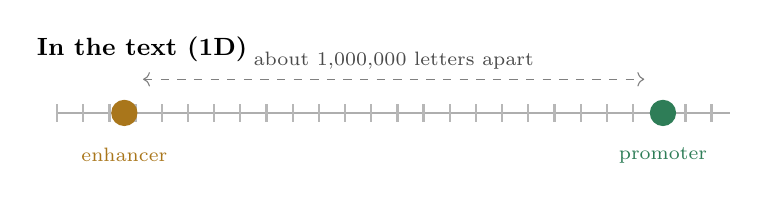
\begin{tikzpicture}[scale=0.95]
% linear
\node[anchor=west, font=\small\bfseries] at (-0.4,1.55) {In the text (1D)};
\draw[line width=1pt, inkgrey!45] (0,0.7) -- (9,0.7);
\foreach \x in {0,0.35,...,9} \draw[inkgrey!40, line width=0.8pt] (\x,0.58) -- (\x,0.82);
\fill[headamber] (0.9,0.7) circle (5pt);
\fill[outgreen]  (8.1,0.7) circle (5pt);
\node[font=\scriptsize, headamber, below=5pt] at (0.9,0.55) {enhancer};
\node[font=\scriptsize, outgreen,  below=5pt] at (8.1,0.55) {promoter};
\draw[<->, inkgrey!70, dashed] (1.15,1.15) -- (7.85,1.15);
\node[font=\scriptsize, inkgrey, above] at (4.5,1.15) {about 1{,}000{,}000 letters apart};
\end{tikzpicture}

\vspace{0.5cm}

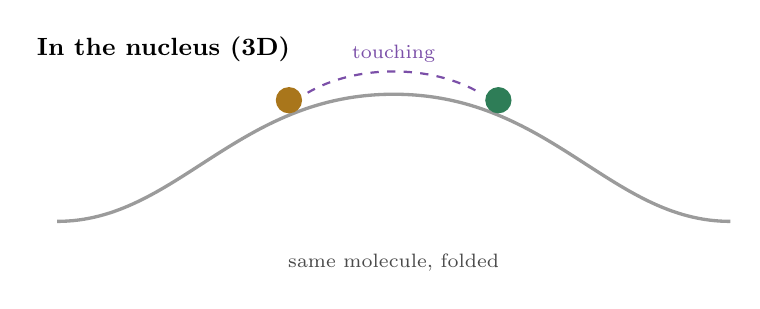
\begin{tikzpicture}[scale=0.95]
\node[anchor=west, font=\small\bfseries] at (-0.4,2.3) {In the nucleus (3D)};
\draw[line width=1.2pt, inkgrey!55]
      (0,0) .. controls (1.6,0) and (2.4,1.7) .. (4.5,1.7)
            .. controls (6.6,1.7) and (7.4,0) .. (9,0);
\fill[headamber] (3.1,1.62) circle (5pt);
\fill[outgreen]  (5.9,1.62) circle (5pt);
\draw[structpurple, thick, dashed] (3.35,1.72) .. controls (4.0,2.1) and (5.0,2.1) .. (5.65,1.72);
\node[font=\scriptsize, structpurple, above] at (4.5,2.0) {touching};
\node[font=\scriptsize, inkgrey] at (4.5,-0.55) {same molecule, folded};
\end{tikzpicture}
\end{center}

That contact is how a distant enhancer reaches its gene. Physical closeness, not
textual closeness, is what decides which enhancer controls which promoter.

\begin{plainbox}
\textbf{Two different meanings of ``near''.}

\emph{Near in sequence} means few letters apart in the text.

\emph{Near in space} means physically touching inside the cell.

They are not the same thing, and it is the second one that controls genes. A
model that only reads the text sees the first one only.
\end{plainbox}

\section{Hi-C: measuring the folding}

We do not have to guess how the genome folds. There is an experiment that
measures it, called \term{Hi-C}.

The idea, simplified to its essentials:

\begin{enumerate}
\item Freeze the DNA in place so that stretches which are touching stay stuck
      together.
\item Cut the DNA into fragments.
\item Glue together the fragment ends that were touching.
\item Read the glued pairs. Each pair says ``these two places in the genome were
      close together''.
\item Count how often each pair of places shows up.
\end{enumerate}

The result is a \term{contact map}: a big table of counts.

\begin{itemize}
\item The genome is chopped into equal-sized \term{bins} --- ours are
      \textbf{\WEbinkb\,kb} each, meaning \WEbinkb{},000 letters.
\item Row $i$ and column $j$ of the table hold the number of times bin $i$ and
      bin $j$ were found touching.
\item A big number means those two regions are often close in space.
\end{itemize}

\begin{plainbox}
\textbf{Two maps of the same territory.}

The \emph{DNA sequence} answers: \emph{what is written in the genome?}

The \emph{Hi-C contact map} answers: \emph{which parts of the genome are
physically close?}

Most DNA models only ever read the first map. This project gives the model both,
and --- this is the part that matters --- lets the second one change how it reads
the first.
\end{plainbox}

\subsection{The single most important property of a contact map}

Contact counts are dominated by one boring fact: \textbf{regions that are close
in the text touch more often, simply because they are attached.} Two bins right
next to each other will have a huge count. Two bins a megabase apart will have a
small one, whether or not anything interesting connects them.

If you plot count against separation you get a steep downward curve. It is
usually written $P(s)$ --- the probability of contact at separation $s$.

\begin{center}
\begin{tikzpicture}[scale=0.9]
\draw[->, inkgrey] (0,0) -- (7.6,0) node[right, font=\scriptsize] {separation $s$};
\draw[->, inkgrey] (0,0) -- (0,3.4) node[above, font=\scriptsize] {contact count};
\draw[seqblue, very thick, domain=0.35:7.2, samples=90] plot (\x, {2.9/(\x^0.85)});
\fill[novelred] (5.2,{2.9/(5.2^0.85)+0.95}) circle (3.2pt);
\node[font=\scriptsize, novelred, right] at (5.35,{2.9/(5.2^0.85)+0.95}) {an actual loop};
\node[font=\scriptsize, seqblue, right] at (2.1,1.75) {the boring background};
\end{tikzpicture}
\end{center}

The interesting biology --- a real enhancer--promoter loop --- is the little bump
sitting \emph{above} that curve. To find it you have to divide the background
out. That step is called \term{distance detrending}, and Section~\ref{sec:detrend}
does it with actual numbers.

\begin{carefulbox}
If you skip detrending, then ``the strongest contacts'' just means ``the nearest
bins'', every time. A model fed those would learn the rule \emph{things close in
the text touch}, which it could already work out from the input, and you would
have measured nothing.

This is the single most common way to accidentally produce a meaningless result
in this field.
\end{carefulbox}

% =====================================================================
\part*{Part II --- The machine learning, starting from nothing}
\addcontentsline{toc}{section}{\textbf{Part II --- The machine learning}}

\section{Turning things into vectors}

A neural network cannot work on the letter \code{A}. It works on numbers. So the
first job is always to turn the thing you care about into a list of numbers.

A \term{vector} is just an ordered list of numbers, like $[0.42,\, 0.15,\, 0.12,\,
0.07]$. The number of entries is its \term{dimension}.

The simplest way to turn a base into a vector is \term{one-hot encoding}: use four
slots, one per letter, and put a 1 in the slot for the letter you have.

\begin{center}
\begin{tabular}{c c c c c}
\toprule
 & \code{A} & \code{C} & \code{G} & \code{T}\\
\midrule
\code{A} & 1 & 0 & 0 & 0\\
\code{C} & 0 & 1 & 0 & 0\\
\code{G} & 0 & 0 & 1 & 0\\
\code{T} & 0 & 0 & 0 & 1\\
\bottomrule
\end{tabular}
\end{center}

An \term{embedding} is a vector that a model has \emph{learned}, rather than one you
wrote down by hand. After training, similar things end up with similar
embeddings. That is the whole point: the vector becomes a compressed summary of
what the model has worked out about that thing.

\begin{plainbox}
An embedding is the model's private summary of something, written as a list of
numbers. Two DNA regions that behave similarly should end up with similar
summaries, even if their letters differ.
\end{plainbox}

\section{Attention, from scratch}
\label{sec:attention}

\term{Attention} is the mechanism that lets one part of the input look at other
parts and decide how much to take from each. Almost every modern language model
is built on it, and our model modifies it, so it is worth understanding properly.

Suppose we have three regions, each with an embedding, and region $i$ wants to
gather information from the others. Attention does it in four steps.

\begin{stepbox}{Step 1 --- ask a question, publish an advertisement}
From each region's embedding we compute three new vectors using three learned
matrices:
\begin{itemize}
\item the \term{query} $\qvec{i}$ --- ``here is what I am looking for'';
\item the \term{key} $\kvec{j}$ --- ``here is what I have to offer'';
\item the \term{value} $\vvec{j}$ --- ``here is the actual content I would hand over''.
\end{itemize}
\end{stepbox}

\begin{stepbox}{Step 2 --- score every candidate}
The score of region $j$ from region $i$'s point of view is the \term{dot product}
$\qvec{i}^\top \kvec{j}$: multiply the two vectors entry by entry, then add up. A
large score means the question and the advertisement match well.
\end{stepbox}

\begin{stepbox}{Step 3 --- turn scores into weights that add to one}
Raw scores can be any size. The \term{softmax} function converts a list of scores
into a list of positive weights summing to $1$, so they can be read as
proportions: exponentiate each score, then divide each by the total.
\end{stepbox}

\begin{stepbox}{Step 4 --- take a weighted average}
The output for region $i$ is the sum of every value vector, each multiplied by
its weight. Regions with high weight contribute most.
\end{stepbox}

\begin{mathbox}
For a query at region $i$ over a set of candidate regions $\mathcal{N}(i)$:
\begin{equation}
a_{ij} \;=\; \frac{\exp\!\big(s_{ij}\big)}{\sum_{m \in \mathcal{N}(i)} \exp\!\big(s_{im}\big)},
\qquad
s_{ij} \;=\; \frac{\qvec{i}^\top \kvec{j}}{\sqrt{d}},
\qquad
\text{output}_i \;=\; \sum_{j \in \mathcal{N}(i)} a_{ij}\, \vvec{j}.
\label{eq:plain-attention}
\end{equation}
Here $d$ is the dimension of the vectors. Dividing by $\sqrt{d}$ keeps the scores
from growing large just because the vectors are long, which would make the
softmax output almost all-or-nothing and stop the model learning.
\end{mathbox}

\begin{carefulbox}
\label{box:shift}
\textbf{Softmax ignores anything added equally to every candidate.}

Suppose you add the same constant $\kappa$ to every score $s_{ij}$ for a fixed
$i$. Then
\[
\frac{e^{\,s_{ij}+\kappa}}{\sum_m e^{\,s_{im}+\kappa}}
= \frac{e^{\kappa} e^{\,s_{ij}}}{e^{\kappa}\sum_m e^{\,s_{im}}}
= \frac{e^{\,s_{ij}}}{\sum_m e^{\,s_{im}}}.
\]
The constant cancels exactly. \textbf{It has no effect whatsoever.}

Remember this. In Section~\ref{sec:bias} it stops being a curiosity and becomes a
bug we had to find --- and it is why one term that appeared in an earlier draft of
this architecture was removed.
\end{carefulbox}

\section{Self-supervised pretraining}

To train a model you normally need labelled examples: an input and the right
answer. Labels are expensive. In genomics they are very expensive, because each
one is an experiment.

\term{Self-supervised learning} avoids this by hiding part of the input and asking
the model to reconstruct it. The data labels itself.

\begin{plainbox}
Cover up part of what you already have, ask the model to guess it, and score the
guess. No human ever writes down an answer, but the model still gets a right and
wrong on every example.
\end{plainbox}

\term{Pretraining} means doing this on a large amount of data first, to learn general
structure. \term{Fine-tuning} means then adapting the pretrained model to a specific
task with far fewer labels. A \term{foundation model} is a model built to be
pretrained once and reused for many tasks.

\begin{carefulbox}
Our model has roughly 9 million adjustable numbers. Genuine industrial
foundation models have thousands of times more. We call ours a \textbf{compact
pretrained representation model}, and only call it a foundation-model prototype
if it demonstrably transfers to several tasks. Claiming otherwise in a report is
an easy way to lose a reviewer's trust on page one.
\end{carefulbox}

\section{Graphs}

A \term{graph} is a set of things (\term{nodes}) and the connections between them
(\term{edges}). A road map is a graph: cities are nodes, roads are edges.

Edges can carry information of their own. A road has a length and a speed limit;
in our graph an edge will carry how strongly two genomic regions touch and how
far apart they are in the text.

A graph is \term{sparse} when most possible connections are absent. With
\WEwindows{} nodes there are $15$ possible edges; with $128$ nodes there are
$8{,}128$. Keeping all of them is expensive and mostly pointless, because most
pairs of genomic regions never touch. Ours keeps a small chosen subset.

% =====================================================================
\part*{Part III --- The model}
\addcontentsline{toc}{section}{\textbf{Part III --- The model}}

\section{The idea in one picture}

\begin{center}
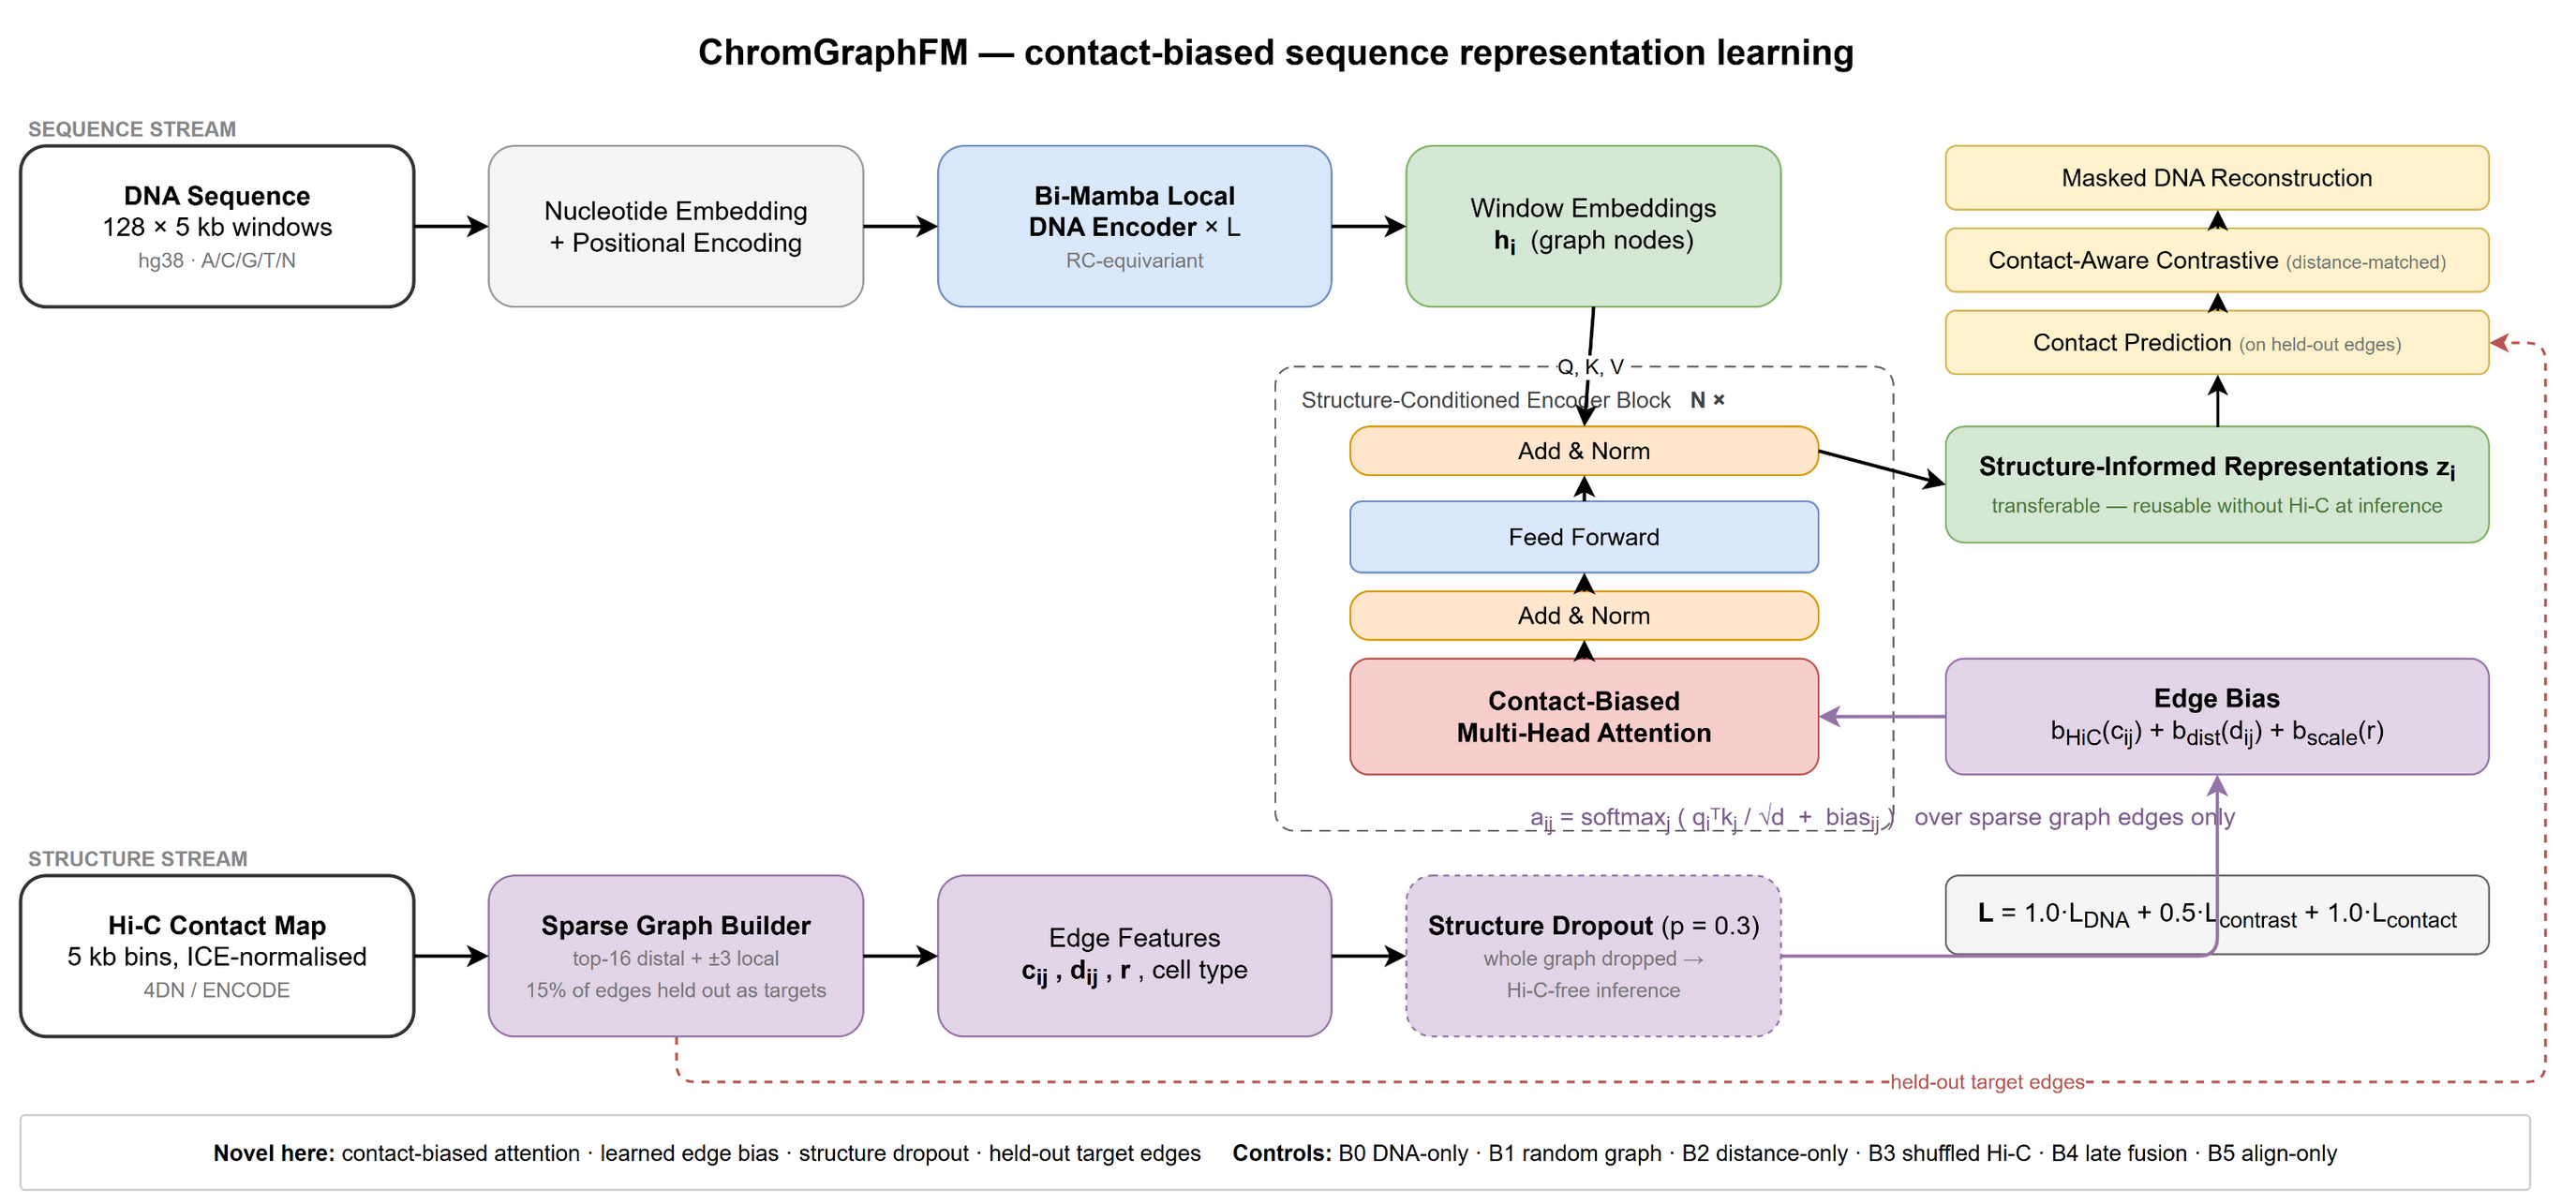
\includegraphics[width=\textwidth]{chromgraphfm_architecture_wide.png}
\end{center}
\captionof{figure}{ChromGraphFM. The upper lane reads DNA; the lower lane turns
Hi-C into a sparse graph. The two meet inside the encoder block, where contact
strength is added to the attention score.}

Read it as two streams that meet in the middle.

\begin{description}[leftmargin=1.6em, style=nextline]
\item[\textcolor{seqblue}{The sequence stream}] cuts the genome into windows, reads
  each one, and produces one vector per window.
\item[\textcolor{structpurple}{The structure stream}] turns the Hi-C map into a
  sparse graph over those same windows.
\item[\textcolor{novelred}{The meeting point}] is attention: the graph decides which
  windows may exchange information, and the contact strengths decide how much.
\end{description}

\begin{whybox}
There are three places you could put Hi-C, and only one of them answers our
question.

\smallskip
\textbf{After the model} (\emph{late fusion}): encode DNA, encode Hi-C, glue the two
summaries together at the end. The DNA representation was already finished before
Hi-C arrived, so Hi-C cannot have shaped it.

\smallskip
\textbf{As the answer} (\emph{prediction target}): train the model to output the
Hi-C map. Useful, but it produces a Hi-C predictor, not a reusable representation
of DNA.

\smallskip
\textbf{Inside the model} (\emph{our approach}): the contact map changes how the DNA
windows talk to each other, at every layer, while the representation is still
being formed.

\smallskip
Only the third one can answer ``does knowing the folding change how the model
reads the sequence?''
\end{whybox}

\section{Step 1 --- windows and nodes}

We cut the region into equal windows of \WEbinkb\,kb --- exactly the same size as
the Hi-C bins.

\begin{whybox}
Making the DNA window and the Hi-C bin the same size is not a detail. If they
differed we would need a pooling layer to convert between them, and every
coordinate calculation would acquire an opportunity to be off by one. Genomics
code fails on off-by-one coordinate errors more than on anything else, and such a
failure is silent: the model still trains, the loss still falls, and the result is
simply wrong.

One window $=$ one bin $=$ one graph node. No conversion, no class of bug.
\end{whybox}

The real model uses $128$ windows at once, covering $640$\,kb. The worked example
in Part IV uses \WEwindows{} windows of \WEbp{} letters so that every number fits
on the page.

\section{Step 2 --- the local encoder}

Each window's DNA goes through an encoder that outputs one vector for the whole
window.

\begin{plainbox}
The encoder reads \WEbinkb{},000 letters and writes a short summary of them ---
in the real model, 256 numbers. It is looking for things like transcription
factor binding motifs, promoter-like patterns, and enhancer-like patterns.

At this stage each window is read \emph{on its own}. No window can see any other
window yet. All communication is saved for the graph.
\end{plainbox}

We use a \term{bidirectional Mamba} encoder. Mamba is a \term{state space model}: it
sweeps along the sequence carrying a running memory, updating it at each letter.

\begin{mathbox}
A state space model keeps a hidden state $\mathbf{s}_t$ and updates it letter by
letter:
\[
\mathbf{s}_t \;=\; \mathbf{A}_t\,\mathbf{s}_{t-1} \;+\; \mathbf{B}_t\, x_t,
\qquad
y_t \;=\; \mathbf{C}_t^\top \mathbf{s}_t .
\]
$x_t$ is the letter at position $t$, $\mathbf{s}_t$ is what the model remembers
after seeing it, and $y_t$ is what it outputs there. In Mamba the matrices
$\mathbf{A}_t, \mathbf{B}_t, \mathbf{C}_t$ depend on the input, which is what lets
the model choose what to remember and what to forget.

The window vector is obtained by averaging the outputs across the window:
$\hvec{i} = \frac{1}{L}\sum_{t=1}^{L} y_t$.
\end{mathbox}

\begin{whybox}
\textbf{Why not attention inside the window too?} Attention costs time
proportional to $L^2$. At $L = 5{,}000$ letters that is 25 million pairs per
window, per layer. A state space model costs time proportional to $L$. That is
the difference between a model that fits on our GPU and one that does not.

\textbf{Why bidirectional?} DNA has no reading direction --- it is double
stranded, and a motif is a motif read either way. A one-directional scan would
throw away half the context for no reason.
\end{whybox}

\section{Step 3 --- building the sparse contact graph}
\label{sec:detrend}

Now the Hi-C map becomes a graph. Four sub-steps.

\begin{stepbox}{3a --- detrend against genomic separation}
For each separation $s$, compute the average count seen at that separation. Then
divide each observed count by the average for its own separation. The result is
called \term{observed over expected}, or O/E.

A value of $1.0$ means ``exactly as much contact as is normal at this distance''.
A value of $2.0$ means twice the normal amount --- something real is going on.
\end{stepbox}

\begin{stepbox}{3b --- squash into a bounded range}
O/E can be any positive number. We map it into $(0,1)$ with
$c = \text{O/E} / (1 + \text{O/E})$, so the bias function later receives a
well-behaved input.
\end{stepbox}

\begin{stepbox}{3c --- keep only a few edges per node}
Each node keeps: all \term{local} neighbours within a small radius along the
sequence, plus its \term{top-$k$} strongest \emph{distal} partners, where distal
means separated by at least a minimum number of bins.
\end{stepbox}

\begin{stepbox}{3d --- hold some edges back as answers}
A fraction of edges is removed from the graph entirely and set aside. The model
never sees them. They become the targets for the contact-prediction objective.
\end{stepbox}

\begin{carefulbox}
Step 3d is not optional bookkeeping. If an edge is both an input to the model and
the thing the model must predict, the model can achieve a perfect score by
copying, and the number you report measures nothing at all.

The held-out edges are chosen with a \emph{fixed} random seed, separate from the
seed used for training. That way every training run sees exactly the same
hold-out, and differences between runs cannot be confused with differences
between hold-outs.
\end{carefulbox}

\section{Step 4 --- contact-biased attention}
\label{sec:bias}

This is the mechanism the project exists to test.

\begin{plainbox}
Ordinary attention decides how much window $i$ should listen to window $j$ using
the DNA alone. We add two more terms before the decision is made:

\begin{itemize}
\item \textbf{how strongly they actually touch} --- pushes the weight up;
\item \textbf{how far apart they are in the text} --- pushes the weight down.
\end{itemize}

Then attention proceeds as normal. The contact map does not get added to the
answer at the end; it changes who is allowed to speak to whom, in every layer,
while the answer is still being formed.
\end{plainbox}

\begin{mathbox}
\begin{equation}
a_{ij} \;=\; \operatorname*{softmax}_{j \in \mathcal{N}(i)}
\left(
\underbrace{\frac{\qvec{i}^\top \kvec{j}}{\sqrt{d}}}_{\text{from the DNA}}
\;+\;
\underbrace{b_{\mathrm{HiC}}(c_{ij})}_{\text{from the contacts}}
\;+\;
\underbrace{b_{\mathrm{dist}}(d_{ij})}_{\text{from the separation}}
\right)
\label{eq:biased-attention}
\end{equation}
with
\begin{itemize}
\item $c_{ij}$ --- the detrended, squashed contact strength between windows $i$ and $j$;
\item $d_{ij} = |i - j|$ --- their separation in bins;
\item $b_{\mathrm{HiC}}$ and $b_{\mathrm{dist}}$ --- small \emph{learned} functions;
\item $\mathcal{N}(i)$ --- the graph neighbours of $i$, and nothing else.
\end{itemize}
\end{mathbox}

\begin{whybox}
\textbf{Why is $b_{\mathrm{dist}}$ there at all, when we already detrended?}

Detrending removed distance from the \emph{edge selection}. But the model still
needs to be able to treat a neighbour 3 bins away differently from one 40 bins
away, because the biology differs. Giving it an explicit, separate distance term
means the two effects can be told apart --- and it is what makes the
distance-only control experiment (Section~\ref{sec:baselines}) constructible:
keep $b_{\mathrm{dist}}$, delete $b_{\mathrm{HiC}}$, and see what is lost.

\smallskip
\textbf{Why learned functions rather than fixed ones?} Because how much a given
contact strength should matter is precisely the thing nobody knows. Fixing it
would be assuming the answer.
\end{whybox}

\begin{carefulbox}
\textbf{A term that did nothing.} An earlier version of this architecture had a
third bias term, $b_{\mathrm{scale}}(r)$, where $r$ was the resolution of the
contact map.

We use a single resolution, so $r$ is the same for every edge, so
$b_{\mathrm{scale}}(r)$ added the same constant to every candidate --- and by
Box~\ref{box:shift} on page~\pageref{box:shift}, softmax cancels it exactly.
The term was mathematically incapable of affecting anything, while sitting in the
headline equation of the project.

It has been removed. It becomes meaningful only if a second resolution is added,
because then $r$ varies between the edges of one node.
\end{carefulbox}

\section{Step 5 --- structure dropout}

During training, with probability $p$, we throw the entire distal graph away for
that sample and let the model work from local edges alone.

\begin{whybox}
The central claim of the project is that the model \emph{internalises} the
structure --- that after pretraining, the DNA encoder is better even when no Hi-C
is available.

To test that, we must run the model without the graph. But if it had never once
experienced life without the graph, removing it at test time would be an input
unlike anything it saw in training, and a poor score would tell us nothing about
what it learned.

Structure dropout makes the no-Hi-C setting a normal, familiar condition.
\end{whybox}

\begin{carefulbox}
Structure dropout \textbf{encourages} robustness. It does not \textbf{guarantee}
that structural knowledge ended up stored in the sequence representation. Whether
that happened is an experimental question, and Section~\ref{sec:hicfree} is the
experiment. Do not write the guarantee into the report.
\end{carefulbox}

\section{Step 6 --- the three training objectives}

The model is trained on three jobs at once.

\subsection{Objective 1 --- rebuild a hidden window}

We blank out one window's summary entirely and ask the model to reconstruct it
from its graph neighbours.

\begin{mathbox}
\begin{equation}
\mathcal{L}_{\mathrm{DNA}}
= \frac{1}{d}\big\| \hat{\mathbf{h}}_{m} - \hvec{m} \big\|^2 ,
\qquad
\hat{\mathbf{h}}_{m} = \text{reconstruct}\big(\{\hvec{j} : j \in \mathcal{N}(m)\}\big)
\end{equation}
where $m$ is the masked window and $\|\cdot\|^2$ is the sum of squared
differences.
\end{mathbox}

\begin{carefulbox}
\textbf{This replaces per-letter masking, and the reason is arithmetic.}

The original plan masked individual bases and reconstructed them from the window
summary $\hvec{i}$. But $\hvec{i}$ is 256 numbers, and a window is 5{,}000 letters
--- 10{,}000 bits of information. You cannot recover 10{,}000 bits from 256
numbers. The objective was not weak, it was \emph{impossible}, and its loss would
have sat flat forever while looking like a training problem.

Masking the whole window and rebuilding it from neighbours is well posed, and it
tests the mechanism more directly: the only route to the answer runs through the
contacts.
\end{carefulbox}

\subsection{Objective 2 --- contacting regions should look alike}

Windows that genuinely touch should get similar representations; windows that do
not should get different ones.

\begin{mathbox}
\begin{equation}
\mathcal{L}_{\mathrm{contrast}}
= -\log
\frac{\exp\!\big(\mathrm{sim}(\zvec{i}, \zvec{j})/\tau\big)}
     {\exp\!\big(\mathrm{sim}(\zvec{i}, \zvec{j})/\tau\big)
      + \sum_{k \in \mathcal{K}} \exp\!\big(\mathrm{sim}(\zvec{i}, \zvec{k})/\tau\big)}
\end{equation}
$(i,j)$ is a touching pair, $\mathcal{K}$ is a set of non-touching ones,
$\mathrm{sim}$ is cosine similarity, and $\tau$ is a temperature controlling how
sharply the model must separate them.
\end{mathbox}

\begin{carefulbox}
\textbf{The negatives must be at the same genomic separation as the positive.}

If you sample them freely, the non-touching pairs will on average be further
apart than the touching pair. The model can then get a perfect score by measuring
distance --- something it can already read straight off the input --- and you will
have learned nothing about 3D structure.

Distance matching is not a refinement here. It is the difference between an
experiment and a non-experiment.
\end{carefulbox}

\subsection{Objective 3 --- predict the contacts we hid}

For each held-out edge, predict its strength from the two window representations
and their separation.

\begin{mathbox}
\begin{equation}
\hat{c}_{ij} = \sigma\!\big(g(\zvec{i}, \zvec{j}, d_{ij})\big),
\qquad
\mathcal{L}_{\mathrm{contact}}
= -\Big[c_{ij}\log \hat{c}_{ij} + (1 - c_{ij})\log(1 - \hat{c}_{ij})\Big]
\end{equation}
$g$ is a small network, and $\sigma(x) = 1/(1+e^{-x})$ squashes its output into
$(0,1)$ so it can be compared with $c_{ij}$.
\end{mathbox}

\subsection{Putting them together}

\begin{mathbox}
\begin{equation}
\mathcal{L}
= \lambda_{\mathrm{DNA}}\,\mathcal{L}_{\mathrm{DNA}}
+ \lambda_{\mathrm{contrast}}\,\mathcal{L}_{\mathrm{contrast}}
+ \lambda_{\mathrm{contact}}\,\mathcal{L}_{\mathrm{contact}}
\end{equation}
with $\lambda_{\mathrm{DNA}} = \WElamdna$,
$\lambda_{\mathrm{contrast}} = \WElamcon$,
$\lambda_{\mathrm{contact}} = \WElamcontact$, tuned on validation chromosomes
only.
\end{mathbox}

% =====================================================================
\part*{Part IV --- One sample, all the way through}
\addcontentsline{toc}{section}{\textbf{Part IV --- Worked example}}

\section{The setting}

Everything in this part is real arithmetic on a deliberately tiny model, so that
you can check any step with a calculator. Every number is produced by
\code{docs/worked\_example.py} and inserted here automatically --- none was typed
by hand.

\begin{center}
\begin{tabular}{l r r}
\toprule
& \textbf{This example} & \textbf{The real model}\\
\midrule
Windows per sample        & \WEwindows & 128\\
Letters per window        & \WEbp & 5{,}000\\
Vector dimension $d$      & \WEdim & 256\\
Attention heads           & 1 & 8\\
Local radius              & 1 & 3\\
Distal edges per node     & 1 & 16\\
\bottomrule
\end{tabular}
\end{center}

\subsection{The DNA}

\begin{center}
\begin{tabular}{c l l}
\toprule
\textbf{Window} & \textbf{Sequence} & \textbf{Note}\\
\midrule
0 & \code{\WEdnaZero}  & \\
1 & \code{\WEdnaOne}   & carries a CTCF-like motif core, \code{CCCTC}\\
2 & \code{\WEdnaTwo}   & \textbf{the window we will follow}\\
3 & \code{\WEdnaThree} & \\
4 & \code{\WEdnaFour}  & \\
5 & \code{\WEdnaFive}  & carries the reverse complement, \code{GAGGG}\\
\bottomrule
\end{tabular}
\end{center}

Windows 1 and 5 are the interesting pair. In real chromatin, a CTCF motif and its
reverse complement facing each other is the classic signature of a loop anchor.
We have built that into the toy so there is something true for the model to find.

\section{Stage 1 --- DNA becomes vectors}

Window \WEfocus{} is \code{\WEdnaTwo}. One-hot encoded, then reduced to base
composition (what fraction of the window is each letter):

\[
\mathbf{f}_{\WEfocus} =
\begin{bmatrix} \WEcompTwoZero \\ \WEcompTwoOne \\ \WEcompTwoTwo \\ \WEcompTwoThree \end{bmatrix}
\quad
\begin{array}{l}
\leftarrow\ \text{A} \\ \leftarrow\ \text{C} \\ \leftarrow\ \text{G} \\ \leftarrow\ \text{T}
\end{array}
\]

Passing this through the encoder gives the window vector:
\[
\hvec{\WEfocus} = \tanh(\mathbf{W}_{\text{enc}} \mathbf{f}_{\WEfocus} + \mathbf{b}_{\text{enc}})
= \begin{bmatrix} \WEhTwoZero & \WEhTwoOne & \WEhTwoTwo & \WEhTwoThree \end{bmatrix}^\top
\]

\begin{carefulbox}
The real encoder is a bidirectional Mamba stack, and its arithmetic cannot be
done on paper. Here it is replaced by the simplest function of the same
\emph{type} --- DNA in, one vector out --- so that the rest of the trace stays
checkable. Everything after this point is the real mechanism, unchanged.
\end{carefulbox}

\section{Stage 2 --- Hi-C becomes contact strengths}

The raw counts for a few pairs, the average at each separation, and the result of
dividing one by the other:

\begin{center}
\begin{tabular}{c c r r r r}
\toprule
\textbf{Pair} & \textbf{Separation} & \textbf{Raw count} & \textbf{Expected} &
\textbf{O/E} & \textbf{$c_{ij}$}\\
\midrule
$(0,1)$ & 1 & \WErawZeroOne & \WEexpOne  & \WEoeZeroOne & \WEcZeroOne\\
$(1,2)$ & 1 & \WErawOneTwo  & \WEexpOne  & \WEoeOneTwo  & \WEcOneTwo\\
$(2,3)$ & 1 & \WErawTwoThree& \WEexpOne  & \WEoeTwoThree& \WEcTwoThree\\
$(1,3)$ & 2 & \WErawOneThree& \WEexpTwo  & \WEoeOneThree& \WEcOneThree\\
$(2,4)$ & 2 & \WErawTwoFour & \WEexpTwo  & \WEoeTwoFour & \WEcTwoFour\\
$(0,5)$ & 5 & \WErawZeroFive& \WEexpFive & \WEoeZeroFive& \WEcZeroFive\\
\textbf{(1,5)} & \textbf{4} & \textbf{\WErawOneFive} & \WEexpFour &
\textbf{\WEoeOneFive} & \textbf{\WEcOneFive}\\
\bottomrule
\end{tabular}
\end{center}

\begin{plainbox}
Look at the raw count for $(1,5)$ against $(0,1)$. In raw terms the neighbouring
pair $(0,1)$ wins easily --- of course it does, they are adjacent.

Now look at the O/E column. Pair $(1,5)$ has far more contact than is normal for
things that far apart. \textbf{Detrending is what makes the loop visible.} Before
it, the loop is buried; after it, the loop is the largest number in the table.
\end{plainbox}

\section{Stage 3 --- the graph}

Local edges (radius 1), then each node's single strongest distal partner:

\begin{center}
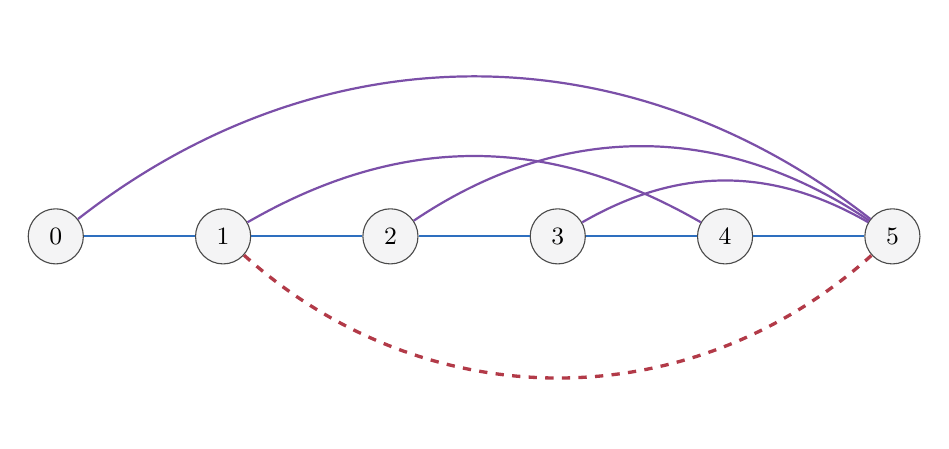
\begin{tikzpicture}[scale=1.25]
\foreach \i in {0,...,5} {
  \node[circle, draw=inkgrey, fill=softgrey, minimum size=7mm,
        font=\small] (n\i) at (\i*1.7,0) {\i};
}
\foreach \i/\j in {0/1,1/2,2/3,3/4,4/5}
  \draw[seqblue, thick] (n\i) -- (n\j);
\draw[structpurple, thick] (n0) to[bend left=38] (n5);
\draw[structpurple, thick] (n1) to[bend left=30] (n4);
\draw[structpurple, thick] (n2) to[bend left=34] (n5);
\draw[structpurple, thick] (n3) to[bend left=30] (n5);
\draw[novelred, very thick, dashed] (n1) to[bend right=42] (n5);
\end{tikzpicture}

\smallskip
{\small
\textcolor{seqblue}{\rule[0.55ex]{1.1em}{1pt}}~local edges \qquad
\textcolor{structpurple}{\rule[0.55ex]{1.1em}{1pt}}~distal edges kept \qquad
\textcolor{novelred}{\rule[0.55ex]{0.35em}{1pt}\,\rule[0.55ex]{0.35em}{1pt}}~edge
$(\WEheldi,\WEheldj)$, held out as the answer}
\end{center}

That leaves \WEnedges{} edges in the conditioning graph. The window we are
following, window \WEfocus{}, has neighbours \textbf{\WEnbrs}.

\begin{plainbox}
Note what just happened. Window \WEfocus{} can now talk to window \WEheldj{},
which is three bins away, because the Hi-C says they touch. A model reading the
text alone would have no reason to connect them.
\end{plainbox}

\section{Stage 4 --- contact-biased attention, in full}

Window \WEfocus{} now gathers information from its three neighbours. We compute
each part of Equation~\eqref{eq:biased-attention} separately.

\subsection{4a --- the DNA part of the score}

The query for window \WEfocus{} is
$\qvec{\WEfocus} = [\,\WEqZero,\ \WEqOne,\ \WEqTwo,\ \WEqThree\,]$, and the scores
against each neighbour's key are $\qvec{\WEfocus}^\top \kvec{j} / \sqrt{\WEdim}$:

\begin{center}
\begin{tabular}{c r r r r}
\toprule
\textbf{Neighbour $j$} & \textbf{DNA score} & $\mathbf{b_{\mathrm{HiC}}}$ &
$\mathbf{b_{\mathrm{dist}}}$ & \textbf{total}\\
\midrule
1 & \WEscoreOne   & \WEbhicOne   & \WEbdistOne   & \WElogitOne\\
3 & \WEscoreThree & \WEbhicThree & \WEbdistThree & \WElogitThree\\
5 & \WEscoreFive  & \WEbhicFive  & \WEbdistFive  & \WElogitFive\\
\bottomrule
\end{tabular}
\end{center}

\begin{plainbox}
The DNA scores are all tiny --- between $\WEscoreFive$ and $\WEscoreOne$. At the
start of training the encoder has learned nothing, so the sequence has almost
nothing to say about who should talk to whom.

The two bias terms are between ten and thirty times larger. \textbf{At the
beginning of training, the structure is doing nearly all of the deciding.} As
training proceeds and the DNA scores grow, the balance shifts. That is exactly
the behaviour we want: start from what was measured, learn your way towards what
can be read from sequence.
\end{plainbox}

For this example the bias functions are kept linear so they can be
differentiated by hand:
\[
b_{\mathrm{HiC}}(c) = \WEalpha\,c,
\qquad
b_{\mathrm{dist}}(d) = -\WEbeta \log_2(d + 1).
\]

\subsection{4b --- softmax}

Take the largest total ($\WEshift$) off every score first --- this changes nothing
mathematically, by Box~\ref{box:shift}, but stops $e^x$ from overflowing on a
computer. Then exponentiate, sum, divide:

\begin{center}
\begin{tabular}{c r r r}
\toprule
\textbf{Neighbour $j$} & \textbf{total $-$ max} & $\mathbf{e^{(\cdot)}}$ &
\textbf{weight $a_{\WEfocus j}$}\\
\midrule
1 & $\WElogitOne   - \WEshift$ & \WEexpoOne   & \textbf{\WEattnOne}\\
3 & $\WElogitThree - \WEshift$ & \WEexpoThree & \textbf{\WEattnThree}\\
5 & $\WElogitFive  - \WEshift$ & \WEexpoFive  & \textbf{\WEattnFive}\\
\midrule
  & & sum $=$ \WEexpsum & $1.0000$\\
\bottomrule
\end{tabular}
\end{center}

\begin{plainbox}
Window \WEfocus{} takes \textbf{\WEattnOne} of its incoming information from
window 1, \textbf{\WEattnThree} from window 3, and \textbf{\WEattnFive} from
window 5.

Window 5 has the \emph{strongest} contact of the three
($b_{\mathrm{HiC}} = \WEbhicFive$) but is three bins away rather than one, so its
distance penalty ($\WEbdistFive$) pulls it back down. The two forces work against
each other, exactly as designed.
\end{plainbox}

\begin{checkbox}
Take the three totals from the table in 4a. Subtract $\WEshift$ from each.
Exponentiate. Add them up --- you should get $\WEexpsum$. Divide each by that
total. You should recover $\WEattnOne$, $\WEattnThree$ and $\WEattnFive$, and they
should add to $1$.
\end{checkbox}

\subsection{4c --- the weighted average}

\[
\text{output}_{\WEfocus}
= \WEattnOne\,\vvec{1} + \WEattnThree\,\vvec{3} + \WEattnFive\,\vvec{5}
= \begin{bmatrix}
\WEattnoutZero & \WEattnoutOne & \WEattnoutTwo & \WEattnoutThree
\end{bmatrix}^\top
\]

\section{Stage 5 --- residual connection and normalisation}

We add the attention output back onto the original window vector, then normalise.

\[
\mathbf{u} = \hvec{\WEfocus} + \text{output}_{\WEfocus}
= \begin{bmatrix} \WEuZero & \WEuOne & \WEuTwo & \WEuThree \end{bmatrix}^\top
\]

\begin{plainbox}
\textbf{Why add the original back?} So that information can flow through the
layer untouched if that is the best thing to do. Without this, a layer that is
not useful yet actively destroys what came before, and deep stacks fail to train.

It also matters here for a specific reason: when structure dropout removes the
graph, this residual path is what keeps the block from collapsing.
\end{plainbox}

Normalising means subtracting the mean and dividing by the standard deviation, so
the four numbers have mean $0$ and variance $1$. For $\mathbf{u}$ the mean is
$\WEumu$ and the variance is $\WEuvar$:

\[
\mathbf{u}_{\text{norm}}
= \frac{\mathbf{u} - \WEumu}{\sqrt{\WEuvar + \varepsilon}}
= \begin{bmatrix} \WEunormZero & \WEunormOne & \WEunormTwo & \WEunormThree \end{bmatrix}^\top
\]

with $\varepsilon = 10^{-5}$ present only so that we never divide by zero.

\section{Stage 6 --- feed-forward, and the final representation}

The normalised vector goes through a small two-layer network --- widen to 8
numbers, keep only the positives, project back to 4 --- then another residual and
normalisation. The result is the structure-informed representation of window
\WEfocus{}:

\[
\boxed{\;
\zvec{\WEfocus} = \begin{bmatrix}
\WEzTwoZero & \WEzTwoOne & \WEzTwoTwo & \WEzTwoThree
\end{bmatrix}^\top
\;}
\]

\begin{plainbox}
\textbf{This vector is the product of the whole project.}

It began as \WEbp{} letters of DNA. It now also carries traces of the windows
that physically touch this one --- and it is a fixed-size list of numbers that any
later task can use.

The research question is whether this vector is more useful than the one a
sequence-only model would have produced. Not whether it looks different. Whether
it is \emph{more useful}, on tasks neither model was trained for.
\end{plainbox}

\section{Stage 7 --- the three losses}

\subsection{Contact prediction on the held-out edge}

The model never saw edge $(\WEheldi,\WEheldj)$. Using $\zvec{\WEheldi}$ and
$\zvec{\WEheldj}$:

\begin{center}
\begin{tabular}{l r}
\toprule
Head output (before squashing) & \WElogitc\\
Predicted strength $\hat{c}$   & \WEchat\\
True strength $c$              & \WEctrue\\
\midrule
$\mathcal{L}_{\mathrm{contact}}$ & \textbf{\WElcontact}\\
\bottomrule
\end{tabular}
\end{center}

The model predicted \WEchat{} where the truth was \WEctrue{} --- it badly
under-estimated a real loop. That is expected: none of these weights has been
trained. This number falling over the course of training is the model learning to
read loops out of sequence.

\subsection{Contrastive}

The positive is the touching pair $(\WEheldi,\WEheldj)$, which spans \WEseppos{}
bins. The negatives are the other pairs spanning exactly \WEseppos{} bins:
\WEnegs.

\begin{center}
\begin{tabular}{l r}
\toprule
Similarity of the positive pair & \WEsimpos\\
Similarity of the negative pair & \WEsimnegone\\
Temperature $\tau$              & \WEtau\\
\midrule
$\mathcal{L}_{\mathrm{contrast}}$ & \textbf{\WElcontrast}\\
\bottomrule
\end{tabular}
\end{center}

\begin{carefulbox}
\textbf{Distance matching compares pairs, not partners --- and the first version
of this example got it wrong.}

The obvious reading of ``distance-matched negatives'' is: keep the same anchor,
and pick other partners the same distance away. That fails here. From window
\WEheldi{} at a separation of \WEseppos{} bins there is exactly one partner in a
\WEwindows-window region, and it is the positive. The first draft silently fell
back to a partner at a \emph{different} separation --- which is exactly the bias
the matching exists to remove.

The correct comparison is pair against pair: hold the separation fixed, and ask
whether \emph{this} pair at \WEseppos{} bins looks more like a contact than
\emph{other} pairs at \WEseppos{} bins. \code{docs/verify\_math.py} now asserts
it.
\end{carefulbox}

\subsection{Masked window}

Window \WEmasked{} is blanked and rebuilt from its neighbours:
$\mathcal{L}_{\mathrm{DNA}} = \WEldna$.

\subsection{Total}

\begin{mathbox}
\[
\mathcal{L}
= \WElamdna \times \WEldna
+ \WElamcon \times \WElcontrast
+ \WElamcontact \times \WElcontact
= \boxed{\WEltotal}
\]
\end{mathbox}

\section{Stage 8 --- how the model learns to trust Hi-C}

Training adjusts every number in the model to make $\mathcal{L}$ smaller,
including $\alpha$ --- the slope of $b_{\mathrm{HiC}}$, which controls how much
the contact map is allowed to influence attention at all.

\begin{mathbox}
Differentiating the softmax in Equation~\eqref{eq:biased-attention} with respect
to $\alpha$, where $b_{\mathrm{HiC}}(c) = \alpha c$:
\begin{equation}
\frac{\partial a_{ij}}{\partial \alpha}
= a_{ij}\Big(c_{ij} - \sum_{m \in \mathcal{N}(i)} a_{im} c_{im}\Big)
\label{eq:grad}
\end{equation}
Read it in words: \emph{a neighbour whose contact strength is above the
attention-weighted average gets more weight when $\alpha$ grows; one below it gets
less.}
\end{mathbox}

For window \WEfocus{}, the weighted average contact strength is $\WEmeanc$:

\begin{center}
\begin{tabular}{c r r r}
\toprule
\textbf{$j$} & $c_{\WEfocus j}$ & $c_{\WEfocus j} - \WEmeanc$ &
$\partial a_{\WEfocus j}/\partial \alpha$\\
\midrule
1 & \WEcnbOne   & $\WEcnbOne - \WEmeanc$   & \WEgradOne\\
3 & \WEcnbThree & $\WEcnbThree - \WEmeanc$ & \WEgradThree\\
5 & \WEcnbFive  & $\WEcnbFive - \WEmeanc$  & \WEgradFive\\
\bottomrule
\end{tabular}
\end{center}

These are not zero, so there is a real learning signal: the model can discover for
itself how much the Hi-C is worth.

\begin{carefulbox}
\textbf{This table was zero on the first run, and finding out why mattered.}

The first version of the toy Hi-C was generated purely as a function of
separation. After detrending, every O/E came out at exactly $1.0$, so $c_{ij}$ was
identical for all three neighbours, so $b_{\mathrm{HiC}}$ was a constant --- and
by Box~\ref{box:shift}, softmax cancelled it. The gradient was exactly $0$.

The lesson is not about toy data. \textbf{If the Hi-C carried no information
beyond genomic distance, this mechanism would contribute literally nothing}, and
the model would be mathematically unable to tell you so --- it would simply train
as though the term were absent.

That is precisely what the shuffled-Hi-C control in Section~\ref{sec:baselines} is
built to detect.
\end{carefulbox}

% =====================================================================
\part*{Part V --- How we will know whether it worked}
\addcontentsline{toc}{section}{\textbf{Part V --- Evaluation}}

\section{The controls}
\label{sec:baselines}

A number on its own means nothing. Every arm below is trained with the
\textbf{same} parameter count, data, optimiser, schedule and step budget. Only the
structural signal differs.

\begin{center}
\renewcommand{\arraystretch}{1.25}
\begin{tabular}{@{}l p{4.3cm} p{6.6cm}@{}}
\toprule
\textbf{Arm} & \textbf{What changes} & \textbf{The question it answers}\\
\midrule
\textbf{B0} & No graph at all &
  Does structure help at all, at equal capacity?\\
\textbf{B1} & Edges placed at random &
  Does \emph{any} graph help, regardless of meaning?\\
\textbf{B2} & Edges from separation only &
  Is the gain just distance --- which the model can already read?\\
\textbf{B3} & Real contact values, shuffled &
  Does the actual biology matter? Same statistics, destroyed meaning.\\
\textbf{B4} & Hi-C added after encoding &
  Is conditioning inside the encoder better than gluing on afterwards?\\
\textbf{B5} & Hi-C only as an alignment target &
  Does our mechanism beat the closest published approach?\\
\midrule
\textbf{Ours} & Contact-biased attention & ---\\
\bottomrule
\end{tabular}
\end{center}

\begin{plainbox}
\textbf{B3 is the one that decides the project.} It receives exactly the same
amount of extra input as our model, with the same distribution of values --- only
the pairing between values and edges has been scrambled.

If our model does not beat B3, then whatever helped was not chromatin biology, and
we say so.
\end{plainbox}

\section{Hi-C-free inference --- and a trap in the comparison}
\label{sec:hicfree}

The model is run in three modes at the end:

\begin{center}
\begin{tabular}{l c c l}
\toprule
\textbf{Mode} & \textbf{DNA} & \textbf{Hi-C} & \textbf{What it tests}\\
\midrule
Sequence only & yes & no  & Whether structure got into the DNA representation\\
Joint         & yes & yes & Full multimodal capability\\
Structure only& no  & yes & What the graph alone contributes\\
\bottomrule
\end{tabular}
\end{center}

\begin{carefulbox}
\textbf{The headline comparison must be made with Hi-C switched off for both
sides.}

It is tempting to report our model \emph{with} its graph against the sequence-only
baseline B0. But then our model has been handed part of the answer at test time
and B0 has not. It would win, the win would prove nothing, and a reviewer would
say so in one sentence.

The fair and meaningful comparison is: both models run on sequence alone, with the
only difference being what shaped their weights during pretraining. Numbers
measured with the graph available are still worth reporting --- as an upper bound,
labelled as such.
\end{carefulbox}

\section{What would falsify the claim}

Stated in advance, so it can lose:

\begin{itemize}
\item Our model failing to beat \textbf{B3} (shuffled Hi-C) on long-range contact
      prediction.
\item Our model merely matching \textbf{B2} (distance only) --- meaning it learned
      how far apart windows are, not how they fold.
\item No advantage surviving into sequence-only inference --- meaning we built a
      multimodal predictor, not a better DNA representation.
\end{itemize}

\begin{plainbox}
Any of these outcomes gets reported as measured. A clean negative result on a
well-controlled experiment is a real finding about the limits of the signal. A
positive result from an uncontrolled experiment is not a finding at all.
\end{plainbox}

\section{Honest positioning}

Contact-guided attention is \textbf{not} new. Chromoformer used chromatin
interactions to guide attention for regulatory prediction; GraphReg propagated
genomic features over Hi-C-derived graphs; CHROME uses filtered contact graphs
with graph attention. Evo2HiC, the closest precedent, uses Hi-C to guide
contrastive distillation from a large DNA model into a compact encoder.

\begin{carefulbox}
None of the following may be claimed:
\begin{itemize}
\item the first genomic foundation model to use Hi-C;
\item the first Hi-C foundation model;
\item the first model to combine DNA sequence and Hi-C;
\item the invention of contact-guided attention.
\end{itemize}
Each is contradicted by published work.
\end{carefulbox}

What we do claim is narrower and testable:

\begin{tcolorbox}[colback=softgrey, colframe=deepblue, boxrule=0.6pt, arc=3pt]
A compact, end-to-end, self-supervised model combining a bidirectional Mamba DNA
encoder with sparse Hi-C-conditioned information flow --- evaluated for whether
the resulting DNA representation transfers across genomic tasks and retains
structural information when Hi-C is unavailable at inference.

\smallskip
The contribution is the \emph{integration and its evaluation}, not the individual
components.
\end{tcolorbox}

% =====================================================================
\appendix
\part*{Appendix}
\addcontentsline{toc}{section}{\textbf{Appendix}}

\section{Notation}

\begin{center}
\renewcommand{\arraystretch}{1.3}
\begin{tabular}{@{}c l@{}}
\toprule
\textbf{Symbol} & \textbf{Meaning}\\
\midrule
$i, j$ & indices of genomic windows\\
$\hvec{i}$ & the vector the local encoder produces for window $i$\\
$\zvec{i}$ & the structure-informed representation, after the encoder block\\
$\qvec{i}, \kvec{j}, \vvec{j}$ & query, key and value vectors\\
$d$ & the dimension of those vectors (\WEdim{} here, 256 in the real model)\\
$c_{ij}$ & detrended contact strength between windows $i$ and $j$, in $(0,1)$\\
$d_{ij}$ & their separation, counted in bins\\
$a_{ij}$ & attention weight: how much $i$ takes from $j$\\
$\mathcal{N}(i)$ & the graph neighbours of window $i$\\
$b_{\mathrm{HiC}}, b_{\mathrm{dist}}$ & the learned bias functions\\
$\alpha$ & the slope of $b_{\mathrm{HiC}}$ in the worked example\\
$\tau$ & contrastive temperature\\
$\lambda_\bullet$ & the weight of each loss term\\
$\sigma(x)$ & the logistic function $1/(1+e^{-x})$\\
\bottomrule
\end{tabular}
\end{center}

\section{Glossary}

\begin{description}[leftmargin=0pt, style=nextline, itemsep=3pt]
\item[Base / nucleotide] One letter of DNA: A, C, G or T.
\item[Bin] A fixed-size chunk of the genome used by Hi-C. Ours are \WEbinkb\,kb.
\item[Chromatin] DNA together with the proteins it is wrapped around --- DNA as it
  actually exists in a cell, rather than as an abstract sequence.
\item[Contact map] The table of Hi-C counts: how often each pair of bins was found
  touching.
\item[CTCF] A protein that binds specific DNA motifs and helps anchor chromatin
  loops. Its motif appearing at both ends of a loop is a strong signature.
\item[Detrending] Dividing observed contact counts by the average expected at that
  separation, to remove the background distance effect.
\item[Embedding] A learned vector summary of something.
\item[Enhancer] A DNA region that increases the activity of a gene, often from far
  away.
\item[Foundation model] A model pretrained once on broad data, then reused for many
  tasks.
\item[hg38] The human reference genome assembly this project uses.
\item[Hi-C] The experiment that measures which genomic regions are physically close.
\item[Loop] A chromatin structure bringing two distant genomic regions together.
\item[Mamba] A state space sequence model; costs time proportional to length rather
  than length squared.
\item[Motif] A short recurring DNA pattern that a protein recognises.
\item[O/E] Observed over expected --- a contact count divided by the average at its
  separation.
\item[Promoter] The region just in front of a gene where transcription starts.
\item[Self-supervised learning] Training by hiding part of the input and predicting
  it, requiring no human labels.
\item[Softmax] A function turning a list of scores into positive weights that sum
  to one.
\item[Window] One \WEbinkb\,kb piece of DNA; also one node of our graph.
\end{description}

\section{Reproducing the worked example}

\begin{center}
\begin{tabular}{@{}l l@{}}
\toprule
\textbf{File} & \textbf{What it holds}\\
\midrule
\code{docs/worked\_example.py} & the whole toy forward pass\\
\code{docs/generated/we\_values.tex} & every number in Part IV, as \LaTeX{} macros\\
\code{docs/generated/we\_values.json} & the same values, machine readable\\
\code{docs/verify\_math.py} & 32 numerical checks on the mathematics above\\
\code{configs/base.yaml} & the real model's settings\\
\bottomrule
\end{tabular}
\end{center}

Run \code{python docs/worked\_example.py}, then compile this document twice. Not
one number in Part IV is typed into the \LaTeX{} source, so the write-up cannot
disagree with the arithmetic that produced it.

\code{python docs/verify\_math.py} re-derives the claims made above and checks
them numerically: that the softmax weights sum to one and are shift-invariant,
that a constant $b_{\mathrm{scale}}$ term provably cancels, that
Equation~\eqref{eq:grad} agrees with a central finite difference, that every
LayerNorm output has mean $0$ and variance $1$, that observed-over-expected
averages to $1$ at every separation, that the held-out edge is absent from the
conditioning graph, that the contrastive negatives really are distance-matched,
and that the losses match their stated formulae. All 32 checks pass.

\vfill
\begin{center}
\rule{0.35\textwidth}{0.4pt}\\[4pt]
{\small\itshape Every result table in this project stays marked \texttt{??}\\
until a file under \texttt{results/} produces the number.}
\end{center}

\end{document}
